\documentclass{beamer}
\usepackage{xcolor}
\usepackage{amsmath} 
\usepackage[utf8]{inputenc}

\definecolor{purple1}{RGB}{102, 51, 153}
\definecolor{purple2}{RGB}{153, 102, 204}
\definecolor{purple3}{RGB}{204, 153, 255}

\usetheme{Madrid}
\usecolortheme[named=purple1]{structure}
\usepackage[table]{xcolor}
\usepackage{booktabs}
\usepackage{graphicx}
\usepackage{caption}
\usepackage{subcaption}
\usepackage[most]{tcolorbox}



\title{Food Stastistics of College Students}
\subtitle{MA4240 - Applied Statistics}
\author{\textbf{Contributors:} Chitipotu Kushwanth \and K.D.V.S Aditya \and \\ Tera Keshavardhan Reddy \and Manpurwar Ganesh \and Sai Satwik}
\date{\today}

\AtBeginSection[]{
  \begin{frame}
  \vfill
  \centering
  \begin{beamercolorbox}[sep=8pt,center]{title}
    \usebeamerfont{title}\insertsectionhead\par%
  \end{beamercolorbox}
  \vfill
  \end{frame}
}
\setcounter{tocdepth}{3} % Include subsubsections in the table of contents
\setbeamertemplate{footline}{%
  \leavevmode%
  \ifnum\value{framenumber}=1% check if it's the first page
    \hbox{%
      \begin{beamercolorbox}[wd=.5\paperwidth,ht=2.5ex,dp=1.125ex,leftskip=.3cm,rightskip=.3cm]{title in head/foot}%
        \usebeamerfont{title in head/foot}\insertshorttitle
      \end{beamercolorbox}%
      \begin{beamercolorbox}[wd=.5\paperwidth,ht=2.5ex,dp=1.125ex,leftskip=.3cm,rightskip=.3cm]{author in head/foot}%
        \usebeamerfont{author in head/foot}\insertshortsubtitle\hfill\insertframenumber/\inserttotalframenumber
      \end{beamercolorbox}}%
  \else% for the rest of the pages
    \hbox{%
      \begin{beamercolorbox}[wd=.5\paperwidth,ht=2.5ex,dp=1.125ex,leftskip=.3cm,rightskip=.3cm]{author in head/foot}%
        \usebeamerfont{author in head/foot}\insertshorttitle
      \end{beamercolorbox}%
      \begin{beamercolorbox}[wd=.5\paperwidth,ht=2.5ex,dp=1.125ex,leftskip=.3cm,rightskip=.3cm]{title in head/foot}%
        \usebeamerfont{title in head/foot}\insertsectionhead\hfill\insertframenumber/\inserttotalframenumber
      \end{beamercolorbox}}%
  \fi%
  \vskip0pt%
}

\begin{document}
%----------------------------------------------------------------------------------------
%	PRESENTATION INFORMATION
%----------------------------------------------------------------------------------------



%----------------------------------------------------------------------------------------



%----------------------------------------------------------------------------------------
%	TITLE SLIDE
%----------------------------------------------------------------------------------------

\begin{frame}
	\titlepage % Output the title slide, automatically created using the text entered in the PRESENTATION INFORMATION block above
\end{frame}

%----------------------------------------------------------------------------------------
%	TABLE OF CONTENTS SLIDE
%----------------------------------------------------------------------------------------

% The table of contents outputs the sections and subsections that appear in your presentation, specified with the standard \section and \subsection commands. You may either display all sections and subsections on one slide with \tableofcontents, or display each section at a time on subsequent slides with \tableofcontents[pausesections]. The latter is useful if you want to step through each section and mention what you will discuss.

\begin{frame}
    \frametitle{Presentation Overview }
    
    \tableofcontents % Display sections 1 to 3
\end{frame}





%----------------------------------------------------------------------------------------
%	PRESENTATION BODY SLIDES
%----------------------------------------------------------------------------------------


%------------------------------------------------
%----------------------------------------------------------------------------------------

\subsection{Survey Questions}

\begin{frame}
    \frametitle{Survey Questions}
    
    \begin{block}{Survey Questions}
        \begin{enumerate}
            \item Gender
            \item Type
            \item Place of Origin
            \item Which type of taste do you generally prefer in your food?
            \item Which Indian cuisine do you like the most?
            \item Which cuisine do you like to eat among foreign cuisines?
            \item How adventurous are you when it comes to trying new foods? (On a scale of 0 to 10)
            \item How often do you dine out in a typical week?
            \item On average, how much do you spend on food per month, considering dining out and other related expenses?
            \item Do you prefer having dessert after a meal, and if so, what type of dessert do you typically enjoy?
        \end{enumerate}
    \end{block}

\end{frame}

\section{Food statistics }

\subsection{Type of diet }

\begin{frame}
    \frametitle{Type of diet}\
    \begin{figure}
    \centering
    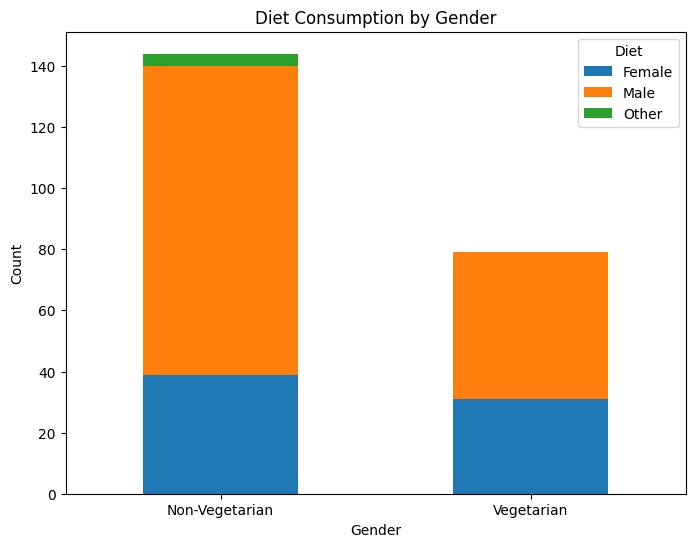
\includegraphics[width=0.7\textwidth]{Veg , Non-veg image.jpg} % Change example-image.jpg to the filename of your image
    \caption{Diet Consumption by Gender} % Caption for the image
    \label{fig:Diet Consumption by Gender} % Label to refer to the image in the text
    \end{figure}
\end{frame}
%------------------------------------------------

\begin{frame}
    \frametitle{Type of diet}\
    This subsection speaks about the proportions of our surveyors that prefer vegetarian and non-vegetarian.
    
    The following are stats related to it.
    
    Let $\pi_1$ denote the proportion of Vegetarians and $\pi_2$ denote the proportion of Non-Vegetarians.
    \begin{align}
        &\text{No. of Vegetarians, } n_{\text{V}} = 79 \\
        &\text{No. of Non-Vegetarians, } n_{\text{NV}} = 144 
    \end{align}
    So,
    \begin{equation}
        \hat{\pi}_1 = \frac{n_{\text{V}}}{n_{\text{V}} + n_{\text{NV}}} = 0.35, \quad \hat{\pi}_2 = \frac{n_{\text{NV}}}{n_{\text{V}} + n_{\text{NV}} } = 0.65
    \end{equation}
\end{frame}
%------------------------------------------------

\begin{frame}
    \frametitle{Confidence interval of ratio of vegetarians }\
    The following formula can be used to calculate the confidence interval of the fraction  of vegetarians 
    \begin{equation}
    \hat{\pi}_1 \pm z_{\frac{\alpha}{2}} \sqrt{\frac{\hat{\pi}_1(1 - \hat{\pi}_1)}{n}}
    \end{equation}
    By substituting, we get,
    \begin{equation}
    0.35 \pm 1.96 \times \sqrt{\frac{0.35(1 - 0.35)}{223}}
    \end{equation}
    
    i.e.,

    \[
    0.35 \pm 0.062 = (0.291, 0.417)
    \]

    
    Thus, we can be 95\% confident that between the ratio of 0.291 and 0.417 of the population on the campus prefers vegetarianism.
    
\end{frame}
%------------------------------------------------
\begin{frame}
    \frametitle{Confidence interval of ratio of Non-Veg }\
    Similarly, by using the same formula, we can calculate the CI for the fraction of non-vegetarians as
    \begin{equation}
    \hat{\pi}_2 \pm z_{\frac{\alpha}{2}} \sqrt{\frac{\hat{\pi}_2(1 - \hat{\pi}_2)}{n}}
    \end{equation}
    Substituting the values, we get
    \begin{equation}
    0.65 \pm 1.96 \times \sqrt{\frac{0.65(1 - 0.65)}{223}}
    \end{equation}
    
    i.e.,

    \[
    0.65 \pm 0.062 = (0.582, 0.708)
    \]

    
    Thus, we can be 95\% confident that between the ratio of 0.582 and 0.708 the population on the campus prefer Non-vegetarian.
    
\end{frame}


%------------------------------------------------


%----------------------------------------------------------------------------------------
\subsection{Taste preferences }
\begin{frame}
    \frametitle{Taste preferences}\
    This subsection speaks about the proportions of our survey related to their taste preferences
    
    The following are stats related to it.
    
    Let $\pi_1$ denote the proportion of people who prefer sweet and $\pi_2$ denote the proportion of people who prefer salt...
    \begin{align}
        &\text{No. of that prefer sweet taste, } n_{\text{1}} = 93 \\
        &\text{No. of that prefer salty taste, } n_{\text{2}} = 54 \\
        &\text{No. of that prefer sour taste, } n_{\text{3}} = 44\\
        &\text{No. of that prefer spicy taste, } n_{\text{4}} = 176 \\
        &\text{No. of that prefer umami taste, } n_{\text{5}} = 21\\
        &\text{No. of people, } n_{\text{T}} = 223
    \end{align}
    So,
    \begin{equation}
        \hat{\pi}_1  = 0.42, \quad \hat{\pi}_2  = 0.25, \quad \hat{\pi}_3  = 0.2, \quad \hat{\pi}_4  = 0.79, \quad \hat{\pi}_5  = 0.09
    \end{equation}
\end{frame}
%------------------------------------------------

\begin{frame}
    \frametitle{Taste preferences }\
    \begin{figure}
    \centering
    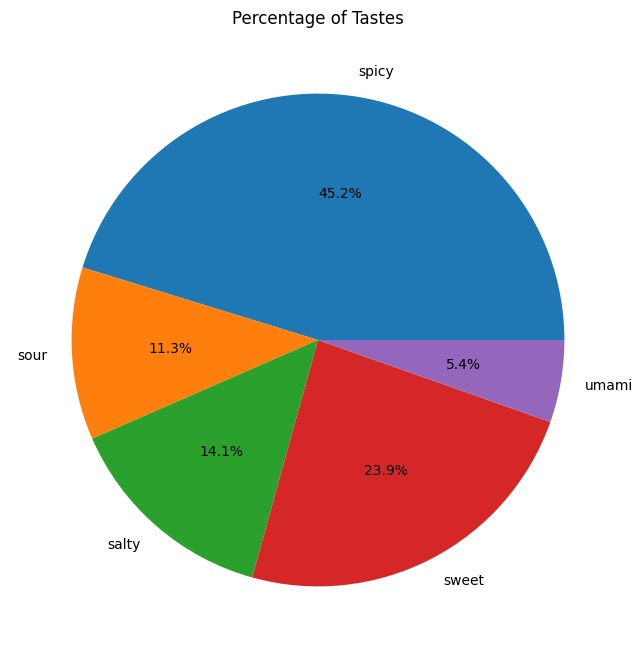
\includegraphics[width=0.5\textwidth]{Distribution of Tastes.jpg} % Change example-image.jpg to the filename of your image
    \caption{Distribution of Tastes} % Caption for the image
    \label{fig:Distribution of Tastes} % Label to refer to the image in the text
    \end{figure}
\end{frame}
%------------------------------------------------

\begin{frame}
    \frametitle{Confidence Interval}\
    \begin{block}{}
    
    For large random samples, a $100(1 - \alpha)\%$ confidence interval for population proportion $p_i$ is:
    
    \[
    \hat{p}_i \pm z_{\frac{\alpha}{2}} \sqrt{\frac{\hat{p}_i(1 - \hat{p}_i)}{n}}
    \quad \text{for } i = 1, 2, 3, 4, 5
    \]
    \end{block}
    The above formula can be used to calculate CI for proportions of people who prefer a particular taste. Applying,It results in the following CIs \\
    
     
    
\end{frame}

%------------------------------------------------

\begin{frame}
    \frametitle{Confidence Interval}
    
    \begin{itemize}
        \item Thus, we can be 95\% confident that between the ratio of 0.352 and 0.482, the population on the campus prefers sweet flavour.
        
        \item Thus, we can be 95\% confident that between the ratio of 0.19 and 0.303, the population on the campus prefers Salty flavour.
        
        \item Thus, we can be 95\% confident that between the ratio of 0.145 and 0.303, the population on the campus prefers Sour flavour.
        
        \item Thus, we can be 95\% confident that between the ratio of 0.736 and 0.843, the population on the campus prefers Spicy flavour.
        
        \item Thus, we can be 95\% confident that between the ratio of 0.056 and 0.133, the population on the campus prefers Umami Flavor.
    \end{itemize}
\end{frame}



%----------------------------------------------------------------------------------------
\subsection{Cuisine preferences }
\begin{frame}
    \frametitle{Cuisine preferences}\
    This subsection speaks about surveyors and their foreign cuisine preferences.
    
    The following are stats related to it.
    
    Let $\pi_1$ denote the proportion of people who prefer sweet and $\pi_2$ denote the proportion of people who prefer salt...
    \begin{align}
        &\text{No. of that prefer Japanese cuisine, } n_{\text{1}} = 63 \\
        &\text{No. of that prefer Italian cuisine, } n_{\text{2}} = 115 \\
        &\text{No. of that prefer Chinese cuisine, } n_{\text{3}} = 135\\
        &\text{No. of that prefer Mexican cuisine, } n_{\text{4}} = 60\\
        &\text{No. of people, } n_{\text{T}} = 223
    \end{align}
    So,
    \begin{equation}
        \hat{\pi}_1  = 0.28, \quad \hat{\pi}_2  = 0.52, \quad \hat{\pi}_3  = 0.60, \quad \hat{\pi}_4  = 0.27
    \end{equation}
\end{frame}
%------------------------------------------------

\begin{frame}
    \frametitle{Cuisine preferences }\
    \begin{figure}
    \centering
    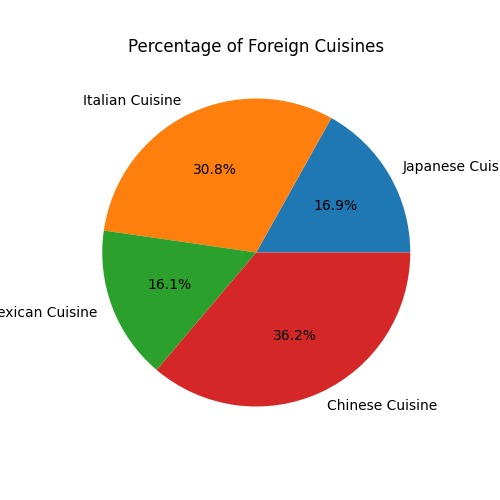
\includegraphics[width=0.5\textwidth]{Percentage of Foreign cuisines.jpg} % Change example-image.jpg to the filename of your image
    \caption{Percentage Distribution of Cuisine} % Caption for the image
    \label{fig:Percentage Distribution of Cuisine} % Label to refer to the image in the text
    \end{figure}
\end{frame}
%------------------------------------------------

\begin{frame}
    \frametitle{Confidence Interval}\
    \begin{block}{}
    For large random samples, a $100(1 - \alpha)\%$ confidence interval for population proportion $p_i$ is:
    
    \[
    \hat{p}_i \pm z_{\frac{\alpha}{2}} \sqrt{\frac{\hat{p}_i(1 - \hat{p}_i)}{n}}
    \quad \text{for } i = 1, 2, 3, 4
    \]
    \end{block}
    Using the above formula, we can get CI for their Proportions related to each Cuisine
    Applying it gives the following outputs: \\
    
     
    
\end{frame}

%------------------------------------------------

\begin{frame}
    \frametitle{Confidence Interval}
    
    \begin{itemize}
        \item Thus, we can be 95\% confident that between the ratio of 0.223 and 0.342, the population on the campus prefers Japanese cuisine.
        
        \item Thus, we can be 95\% confident that between the ratio of 0.45 and 0.581, the population on the campus prefers Italian cuisine.
        
        \item Thus, we can be 95\% confident that between the ratio of 0.541 and 0.67, the population on the campus prefers Chinese cuisine.
        
        \item Thus, we can be 95\% confident that between the ratio of 0.211 and 0.327, the population on the campus prefers Mexican cuisine.
    \end{itemize}
\end{frame}

%----------------------------------------------------------------------------------------
\subsection{Dessert preferences}
\begin{frame}
    \frametitle{Dessert preferences}\
    This subsection speaks about  our surveyors and Their frequency of desert consumption 
    
    The following are stats related to it.
    
    Let $\pi_1$ denote the proportion of people who prefer sweet and $\pi_2$ denote the proportion of people who prefer salt...
    \begin{align}
        &\text{No. of people that prefer dessert often , } n_{\text{1}} = 81 \\
        &\text{No. of people that prefer dessert rarely , } n_{\text{2}} = 116 \\
        &\text{No. of people that do not prefer dessert, } n_{\text{3}} = 26\\
        &\text{No. of people, } n_{\text{T}} = 223
    \end{align}
    So,
    \begin{equation}
        \hat{\pi}_1  = 0.36, \quad \hat{\pi}_2  = 0.52, \quad \hat{\pi}_3  = 0.12
    \end{equation}
\end{frame}
%------------------------------------------------

\begin{frame}
    \frametitle{Dessert preferences }\
    \begin{figure}
    \centering
    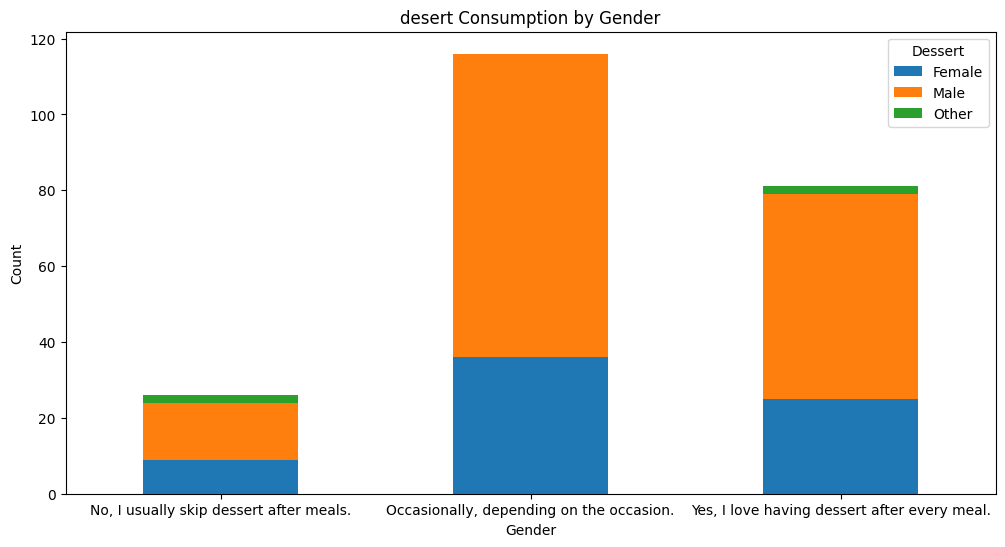
\includegraphics[width=0.7\textwidth]{output_99_0.png} % Change example-image.jpg to the filename of your image
    \caption{ Dessert preference by gender } % Caption for the image
    \label{fig:Percentage Distribution of Cuisine} % Label to refer to the image in the text
    \end{figure}
\end{frame}
%------------------------------------------------
%------------------------------------------------

\begin{frame}
    \frametitle{Dessert preferences }\
    \begin{figure}
    \centering
    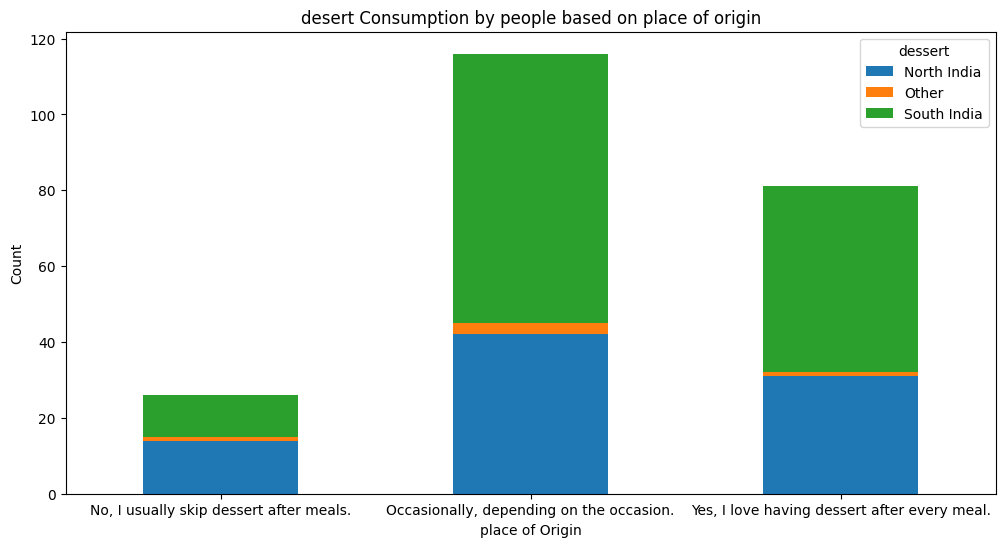
\includegraphics[width=0.7\textwidth]{output_100_0.png} % Change example-image.jpg to the filename of your image
    \caption{ Dessert preference by place of origin } % Caption for the image
    \label{fig:Percentage Distribution of Cuisine} % Label to refer to the image in the text
    \end{figure}
\end{frame}
%------------------------------------------------
\begin{frame}
    \frametitle{Confidence Interval}
    
    \begin{block}{}
    For large random samples, a $100(1 - \alpha)\%$ confidence interval for population proportion $p_i$ is:
    
    \[
    \hat{p}_i \pm z_{\frac{\alpha}{2}} \sqrt{\frac{\hat{p}_i(1 - \hat{p}_i)}{n}}
    \quad \text{for } i = 1, 2, 3
    \]
    \end{block}
    Using the above formula, we can obtain CI for their frequency of dessert consumption.
    Applying the formula, we get the following conclusions:

    
\end{frame}


%------------------------------------------------



\begin{frame}
    \frametitle{Confidence Interval}
    
    \begin{itemize}
        \item We can be  95\% confident that between the ratio of \textbf{0.3 and 0.426}, the population on the campus prefers Dessert \textbf{Often}.
        
        \item We can be  95\% confident that between the ratio of \textbf{0.455 and 0.586}, the population on the campus prefers Dessert \textbf{rarely}.
        
        \item Thus, we can be  95\% confident that between the ratio of \textbf{0.074 and 0.159}, the population on the campus \textbf{does not prefer} having Dessert.
    \end{itemize}
    
\end{frame}


%----------------------------------------------------------------------------------------

\section{Cost statistics }
\subsection{Introduction}
\begin{frame}
    \frametitle{Introduction}\
    
\end{frame}

\begin{frame}
    \frametitle{Introduction }\
    \begin{figure}
    \centering
    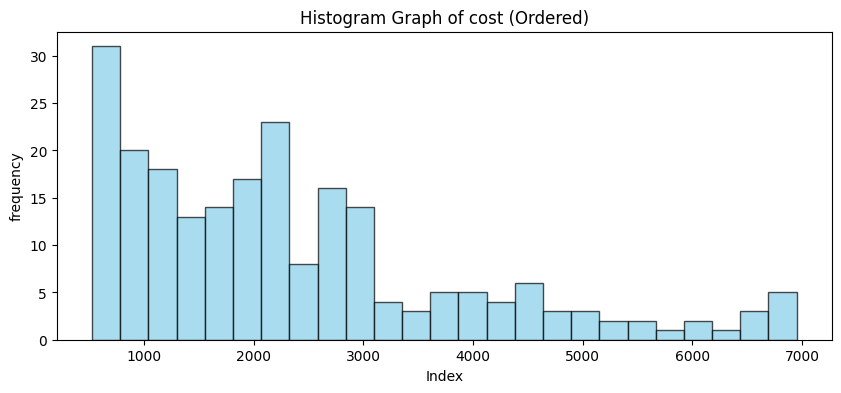
\includegraphics[width=0.8\textwidth]{Histogram for amount spent.png} % Change example-image.jpg to the filename of your image
    \caption{Histogram  for Amount spent } % Caption for the image
    \label{fig:Bar Graph for Costs } % Label to refer to the image in the text
    \end{figure}
\end{frame}

%------------------------------------------------


\begin{frame}
    \frametitle{Overview of Spending statistics}\
    The central tendencies are as follows:
    \begin{block}{}
        \begin{itemize}
            \item \textbf{Count} n:223.000000.
            \item \textbf{Mean} $\bar{x}$ : 2327.668161.
            \item \textbf{Std} S: 1493.292685
            \item \textbf{Min}: 513.000000.
            \item \textbf{25\%}: 1086.000000.
            \item \textbf{50\%}: 2080.000000.
            \item \textbf{75\%}: 2881.500000.
            \item \textbf{Max}: 6900.000000.
        \end{itemize}
    \end{block}
\end{frame}
%------------------------------------------------

\begin{frame}
    \frametitle{Introduction }\
    \begin{figure}
    \centering
    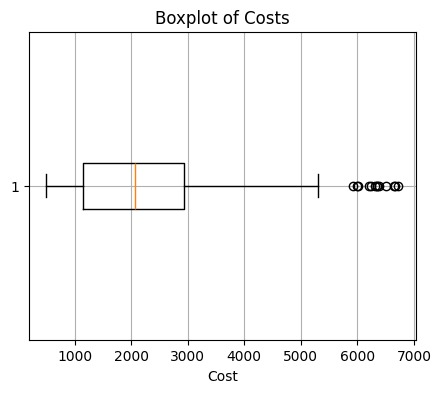
\includegraphics[width=0.6\textwidth]{Boxplots for costs.jpg} % Change example-image.jpg to the filename of your image
    \caption{Box plots for costs } % Caption for the image
    \label{fig:Box plots for costs } % Label to refer to the image in the text
    \end{figure}
\end{frame}

\begin{frame}
    \frametitle{Confidence interval}\
    \begin{block}{}
        If $X_1, X_2, \ldots, X_n$ are normally distributed with unknown mean $\mu$ and variance $\sigma^2$, then a $(1 - \alpha) \times 100\%$ confidence interval for the population mean $\mu$ is:

        \[
        \bar{x} \pm t_{\frac{\alpha}{2}, n-1} \frac{S}{\sqrt{n}}
        \]

    \end{block}
\end{frame}
%------------------------------------------------


\begin{frame}
    \frametitle{Confidence interval}\
    Substitution in the above formula, 
    \begin{align}
    &= 2327.67 \pm 1.97 \frac{1493.29}{\sqrt{223}} \\ &= 2327.67 \pm 196.996 \nonumber \\
    &= (2130.601, 2524.736)
    \end{align}
    Thus, we can say that the mean of money spent by the population of Campus lies in the interval (2130.601, 2524.736)
\end{frame}
%------------------------------------------------
\subsection{Level of Adventurousness}

\begin{frame}
    \frametitle{Level of Adventurousness}
    
    \begin{block}{}
    This part of the project tries to study how Adventurous students are and tries to find out the relation of this to money spent by them.
    \end{block}
    
    \begin{block}{Definition}
    Adventurous in the context of food is their willingness to explore diverse cuisines, flavours, and ingredients, often embracing unconventional or exotic dishes with enthusiasm and curiosity.
    \end{block}
    
    \begin{block}{Categories}
    Four categories of people based on their level of adventurousness are \textbf{low, mid, high, and very high}.
    \end{block}
    
    \begin{block}{Statistics}
    Statistics related to each level are as follows:
    \end{block}
    
\end{frame}

%------------------------------------------------

\begin{frame}
    \frametitle{Level of Adventurousness (Contd.) }\
    \begin{figure}
    \centering
    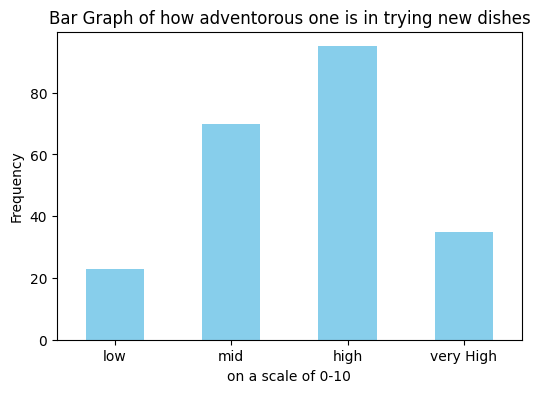
\includegraphics[width=0.7\textwidth]{output_58_0.png} % Change example-image.jpg to the filename of your image
    \caption{Adventurousness level grouped into low,mid,high,very high } % Caption for the image
    \label{fig:Percentage Distribution of Cuisine} % Label to refer to the image in the text
    \end{figure}
\end{frame}

\begin{frame}
    \frametitle{Level of Adventurousness (Contd.) }\
    \begin{figure}
    \centering
    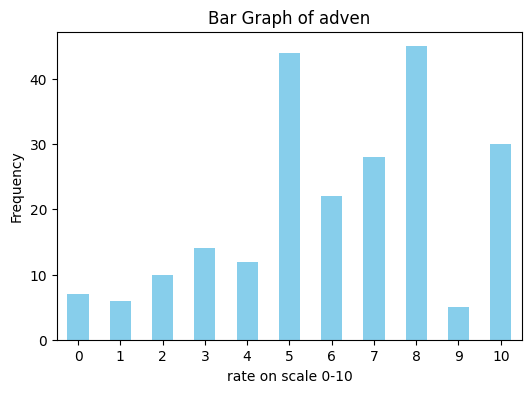
\includegraphics[width=0.7\textwidth]{output_57_0.png} % Change example-image.jpg to the filename of your image
    \caption{Adventurousness level on scale 1-10 } % Caption for the image
    \label{fig:Percentage Distribution of Cuisine} % Label to refer to the image in the text
    \end{figure}
\end{frame}

\begin{frame}
\frametitle{Low}
The central tendencies are as follows:
    \begin{block}{}
        \begin{itemize}
            \item \textbf{Count} n:23.000000.
            \item \textbf{Mean} $\bar{x}$ : 2898.782609.
            \item \textbf{Std} S: 1967.060519
            \item \textbf{Min}: 564.000000.
            \item \textbf{25\%}: 1152.000000.
            \item \textbf{50\%}: 2267.000000.
            \item \textbf{75\%}: 4731.000000.
            \item \textbf{Max}: 6627.000000.
        \end{itemize}
    \end{block}
    Using the following formula we get CI with confidence 95\% as
        \begin{equation}
        \bar{x} \pm t_{\frac{\alpha}{2}, n-1} \frac{S}{\sqrt{n}} =
        2898.78 \pm 2.07 \frac{1967.06}{\sqrt{23}}  = (2048.161,3749.403)
        \end{equation}
        
\end{frame}
%------------------------------------------------

\begin{frame}
\frametitle{Mid}
The central tendencies are as follows:
    \begin{block}{}
        \begin{itemize}
            \item \textbf{Count} n:70.000000.
            \item \textbf{Mean} $\bar{x}$ : 2283.928571.
            \item \textbf{Std} S: 1430.839931
            \item \textbf{Min}: 587.000000.
            \item \textbf{25\%}: 1141.500000.
            \item \textbf{50\%}: 2056.000000.
            \item \textbf{75\%}: 2692.000000.
            \item \textbf{Max}: 6890.000000.
        \end{itemize}
    \end{block}
    Using the following formula we get CI with confidence 95\% as
        \begin{equation}
        \bar{x} \pm t_{\frac{\alpha}{2}, n-1} \frac{S}{\sqrt{n}} =
        2283.92 \pm 1.99 \frac{1430.83}{\sqrt{70}} = (1942.757,2625.100)
        \end{equation}
\end{frame}
%------------------------------------------------

\begin{frame}
\frametitle{High}
The central tendencies are as follows:
    \begin{block}{}
        \begin{itemize}
            \item \textbf{Count} n:95.000000.
            \item \textbf{Mean} $\bar{x}$ : 2271.831579.
            \item \textbf{Std} S: 1435.554846
            \item \textbf{Min}: 513.000000.
            \item \textbf{25\%}: 1086.000000.
            \item \textbf{50\%}: 1935.000000.
            \item \textbf{75\%}: 2963.000000.
            \item \textbf{Max}: 6900.000000.
        \end{itemize}
    \end{block}
    Using the following formula, we get CI with confidence 95\% as
        \begin{equation}
        \bar{x} \pm t_{\frac{\alpha}{2}, n-1} \frac{S}{\sqrt{n}} =
        2271.83 \pm 1.985 \frac{1435.55}{\sqrt{95}}  = (1979.394,2564.269)
        \end{equation}
\end{frame}

\begin{frame}
\frametitle{Very High}
       \begin{block}{}
        \begin{itemize}
            \item \textbf{Count} n:35.000000
            \item \textbf{Mean} $\bar{x}$ : 2191.400000.
            \item \textbf{Std} S: 1397.002931
            \item \textbf{Min}: 549.000000.
            \item \textbf{25\%}: 934.500000.
            \item \textbf{50\%}: 2161.000000.
            \item \textbf{75\%}: 2638.000000.
            \item \textbf{Max}: 5263.000000.
        \end{itemize}
    \end{block}
    Using the following formula, we get CI with confidence 95\% as
        \begin{equation}
        \bar{x} \pm t_{\frac{\alpha}{2}, n-1} \frac{S}{\sqrt{n}} =
        2191.40 \pm 2.032 \frac{1397.0}{\sqrt{35}} = (1722.545,2660.255)
        \end{equation}
\end{frame}
%------------------------------------------------
\begin{frame}
    \frametitle{Confidence intervals}
    From the respective calculations, we can see that:
    \begin{itemize}
        \item The mean of money spent by people that fall into the category of \textbf{low adventurous level} will lie in the interval \textbf{(2048.161, 3749.403)} with a confidence of \textbf{95\%}.
        
        \item The mean of money spent by people that fall into the category of \textbf{mid-adventurous level} will lie in the interval \textbf{(1942.757, 2625.100)} with a confidence of \textbf{95\%}.
        
        \item The mean of money spent by people that fall into the category of \textbf{high adventurous level} will lie in the interval \textbf{(1979.394, 2564.269)} with a confidence of \textbf{95\%}.
        
        \item The mean of money spent by people that fall into the category of \textbf{very high adventurous level} will lie in the interval \textbf{(1722.545, 2660.255)} with a confidence of \textbf{95\%}.
    \end{itemize}
\end{frame}

%------------------------------------------------

\subsection{Dine out }
\begin{frame}
\frametitle{Dine out}
    This part studies the number of days our campus students dine out per week. 
    \begin{block}{}
        \begin{itemize}
            \item \textbf{Count} n:223.000000
            \item \textbf{Mean} $\bar{x}$ : 2.726457.
            \item \textbf{Std} S: 1.977707
            \item \textbf{Min}: 0.000000.
            \item \textbf{25\%}: 1.000000.
            \item \textbf{50\%}: 2.000000.
            \item \textbf{75\%}: 4.000000.
            \item \textbf{Max}: 7.000000.
        \end{itemize}
    \end{block}
     
\end{frame}
%------------------------------------------------
\begin{frame}
    \frametitle{Dine out (Contn.) }\
    \begin{figure}
    \centering
    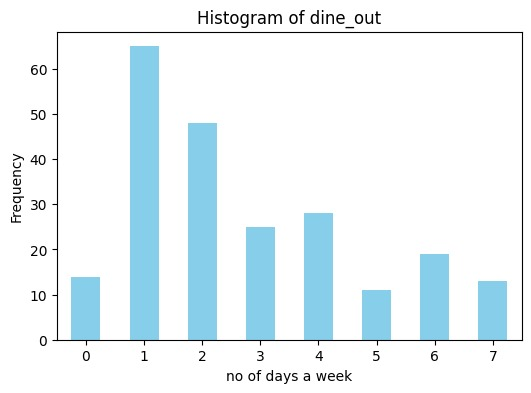
\includegraphics[width=0.7\textwidth]{Histogram of Dine Out.jpg} % Change example-image.jpg to the filename of your image
    \caption{Histogram of Dine Out } % Caption for the image
    \label{fig:Histogram of Dine Out } % Label to refer to the image in the text
    \end{figure}
\end{frame}


\begin{frame}
\frametitle{Dine out (Contn.)}
    
    Using the following formula, we get CI with confidence 95\% as
        \begin{equation}
        \bar{x} \pm t_{\frac{\alpha}{2}, n-1} \frac{S}{\sqrt{n}} =
        2.73 \pm 1.970 \frac{1.977}{\sqrt{223}} = (2.465,2.987)
        \end{equation}
    Thus, the average number of days of dining out of our campus students falls in the interval (2.465,2.987) with a confidence of 95\%  
\end{frame}

%------------------------------------------------



\begin{frame}
    \frametitle{CIs for difference of two population proportions}\
    \begin{block}{}
    For large random samples, an approximate $100(1 - \alpha)\%$ confidence interval for the difference in two population proportions $p_1 - p_2$ is:

    \[
    (\hat{p}_1 - \hat{p}_2) \pm z_{\frac{\alpha}{2}} \sqrt{\frac{\hat{p}_1(1 - \hat{p}_1)}{n_1} + \frac{\hat{p}_2(1 - \hat{p}_2)}{n_2}}
    \]
    \end{block}

    Substituting in the formula, we get
    \begin{equation}
    (0.35 - 0.40) \pm 1.96 \sqrt{\frac{0.50 \times 0.50}{400} + \frac{0.40 \times 0.60}{250}}
    \end{equation}
    
    which simplifies to
    
    \begin{equation}
    0.10 \pm 0.078 = (0.022, 0.178)
    \end{equation}
  
\end{frame}
%------------------------------------------------
%----------------------------------------------------------------------------------------


%----------------------------------------------------------------------------------------
\section{Hypothesis Testing }

\subsection{Hypothesis - 1}

\begin{frame}
    \frametitle{Hypothesis - 1}
    \begin{block}{Hypothesis}
        The proportion of vegetarians who prefer dessert after meals is higher than the proportion of non-vegetarians who prefer dessert after meals
    \end{block}
    Let $\pi_1$ denote the proportion of Vegetarians preferring dessert after meals and $\pi_2$ denote the proportion of Non-Vegetarians preferring dessert after meals.
    \begin{align}
        &\text{No. of Vegetarians in sampled data, } n_{\text{V}} = 49 \\
        &\text{No. of Non-Vegetarians in sampled data, } n_{\text{NV}} = 100 \\
        &\text{No. of Vegetarians preferring dessert, } n_{\text{Vp}} = 23 \\
        &\text{No. of Non-Vegetarians preferring dessert, } n_{\text{NVp}} = 30
    \end{align}
    So,
    \begin{equation}
        \hat{\pi}_1 = \frac{n_{\text{Vp}}}{n_{\text{V}}} = 0.47, \quad \hat{\pi}_2 = \frac{n_{\text{NVp}}}{n_{\text{NV}}} = 0.30
    \end{equation}
\end{frame}
%------------------------------------------------
\begin{frame}
    \frametitle{Hypothesis - 1}
    Now,
    \begin{align}
        H_0 &: \pi_1 - \pi_2 \leq 0 \\
        H_a &: \pi_1 - \pi_2 > 0
    \end{align}
    Now, we check the conditions:
    \begin{align}
        n_1\hat{\pi}_1 &\geq 5, \quad n_1(1 - \hat{\pi}_1) \geq 5 \\
        n_2\hat{\pi}_2 &\geq 5, \quad n_2(1 - \hat{\pi}_2) \geq 5
    \end{align}
    So, the test statistic is
    \begin{equation}
        Z = \frac{\hat{\pi}_1 - \hat{\pi}_2}{\sqrt{\frac{\hat{\pi}_1(1-\hat{\pi}_1)}{n_1} + \frac{\hat{\pi}_2(1-\hat{\pi}_2)}{n_2}}} = 2.00
    \end{equation}
    and
    \begin{equation}
        z_{0.05} = 1.645
    \end{equation}
\end{frame}
%-----------------------------------------------------------------------------
\begin{frame}
\frametitle{Hypothesis - 1}
\textbf{Rejection Region approach:}
We will reject $H_0$ if the test statistic $Z > Z_{\alpha}$.
With a significance level $\alpha = 0.05$, $z_{0.05} < Z$.
Since $Z > z_{0.05}$, which means it's lying in the rejection region, so we will reject $H_0$.

\begin{block}{Inference} We can infer that, statistically with a significance level of $0.05$, The proportion of vegetarians who prefer dessert after meals is higher  than the proportion of non-vegetarians who prefer dessert after meals
 \end{block}

\end{frame}
%----------------------------------------------------------------------------------------
\subsection{Hypothesis - 2}

\begin{frame}
    \frametitle{Hypothesis - 2}
    \begin{block}{Hypothesis}
       The mean expenditure on food per month by females is greater than the mean expenditure on food per month by males
    \end{block}
    From the data sampled from the whole data, we have the mean amount spent by males ($x_m$) and females ($x_f$) as follows,
    \[ x_m = 2380.65 \]
    \[ x_f = 2593.78 \]
    Since we have $x_f > x_m$, we will do Hypothesis Testing with,
\end{frame}
%------------------------------------------------

\begin{frame}
    \frametitle{Hypothesis - 2}
    \begin{align}
        H_0 &: \mu_f - \mu_m \leq 0 \\
        H_a &: \mu_f - \mu_m > 0
    \end{align}
    
    From the data we got,
    \[ S_f = 1619.76 \]
    \[ S_m = 1702.65 \]
    \[ \Rightarrow \frac{1}{2} < \frac{S_f}{S_m} \approx 0.95 < 2.0 \]
    
    So we assume population variances to be the same and then pooled variance will be equal to ($n_f = 50$, $n_m = 100$),
    \begin{equation}
        S_p = \sqrt{\frac{99 \times 1702.65 \times 1702.65 + 49 \times 1619.76 \times 1619.76}{148}} \approx  = 1647.668
    \end{equation}
\end{frame}
%------------------------------------------------
\begin{frame}
    \frametitle{Hypothesis - 2}
    The test statistic will be,
    \begin{align}
        t &= \frac{(x_f - x_m) - 0}{S_p \sqrt{\frac{1}{n_f} + \frac{1}{n_m}}} \\
        &= \frac{2667.83 -2259.61}{ 1647.668\times 0.173} \\
        & = 0.747
    \end{align}
\end{frame}
%-----------------------------------------------------------------------------
\begin{frame}
    \frametitle{Hypothesis - 2}
    \textbf{Rejection Region Approach:}
We will reject \( H_0 \) if the test statistic \( t > t_{\alpha,n_f+n_m-2} \) with \( \alpha = 0.05 \) (Significance Level),
\( t_{0.05,188} = 1.655 \).
The observed test statistic (0.747) is less than 1.655, hence it isn't in the rejection region.

\begin{block}{Inference} We can infer that, statistically with a significance level of $0.05$, The mean expenditure on food per month by females may not be greater than the mean expenditure on food per month by males
 \end{block}
 
\end{frame}
%----------------------------------------------------------------------------------------
\subsection{Hypothesis - 3}

\begin{frame}
    \frametitle{Hypothesis - 3}
    
    \begin{block}{Hypothesis}
       The proportion of South Indians who prefer their regional cuisine is higher than the proportion of North Indians who prefer their regional cuisine
    \end{block}
    Let $\pi_1$ denote the proportion of South Indian people preferring South cuisine and $\pi_2$ denote the proportion of North Indian people preferring North cuisine.
    \begin{align}
        &\text{No. of South Indians in sampled data, } n_{\text{S}} = 100 \\
        &\text{No. of North Indians in sampled data, } n_{\text{N}} = 50 \\
        &\text{No. of South Indians preferring South cuisine, } n_{\text{Sp}} = 83 \\
        &\text{No. of North Indians preferring North cuisine, } n_{\text{Np}} = 24
    \end{align}
    
    So,
    \begin{equation}
        \hat{\pi}_1 = \frac{n_{\text{Sp}}}{n_{\text{S}}} = 0.83, \quad \hat{\pi}_2 = \frac{n_{\text{Np}}}{n_{\text{N}}} = 0.48
    \end{equation}
\end{frame}
%------------------------------------------------
\begin{frame}
    \frametitle{Hypothesis - 3}
    Now,
    \begin{align}
        H_0 &: \pi_1 - \pi_2 \leq 0 \\
        H_a &: \pi_1 - \pi_2 > 0
    \end{align}
    Now, we check the conditions:
    \begin{align}
        n_1\hat{\pi}_1 &\geq 5, \quad n_1(1 - \hat{\pi}_1) \geq 5 \\
        n_2\hat{\pi}_2 &\geq 5, \quad n_2(1 - \hat{\pi}_2) \geq 5
    \end{align}
    So, the test statistic is
    \begin{equation}
        Z = \frac{\hat{\pi}_1 - \hat{\pi}_2}{\sqrt{\frac{\hat{\pi}_1(1-\hat{\pi}_1)}{n_1} + \frac{\hat{\pi}_2(1-\hat{\pi}_2)}{n_2}}} = 4.38
    \end{equation}
    and
    \begin{equation}
        z_{0.05} = 1.645
    \end{equation}
    
\end{frame}
%-----------------------------------------------------------------------------
\begin{frame}
    \frametitle{Hypothesis - 3}
    \textbf{Rejection Region approach:}
We will reject $H_0$ if the test statistic $Z > Z_{\alpha}$.
With a significance level $\alpha = 0.05$, $z_{0.05} < Z$.
Since $Z > z_{0.05}$, which means it's lying in the rejection region, so we will reject $H_0$.

\begin{block}{Inference} We can infer that, statistically with a significance level of $0.05$,  The proportion of South Indians who prefer their regional cuisine is higher than the proportion of North Indians who prefer their regional cuisine
 \end{block}

    
\end{frame}
%----------------------------------------------------------------------------------------
\subsection{Hypothesis - 4}

\begin{frame}
    \frametitle{Hypothesis - 4}
    \begin{block}{Hypothesis}
        The number of people who prefer Japanese cuisine is greater than the number of people who do not prefer it
    \end{block}
    From the data collected, 
    \begin{align}
        &\text{No. of People preferring Japanese Cuisine in sampled data, } n_{\text{J}} = 28 \\
        &\text{Total people in sampled data, } n_{\text{n}} = 100 \\
    \end{align}
    
    The estimated proportion is,
    \begin{equation}
        \hat{\pi} = \frac{n_{\text{J}}}{n_{\text{n}}} = 0.28
    \end{equation}
    
    Let $\pi$ denote the proportion of people preferring Japanese Cuisine. Here,
    \begin{equation}
        H_0: \pi \leq 0.5 \quad \text{vs.} \quad H_a: \pi > 0.5
    \end{equation}
\end{frame}
%------------------------------------------------
\begin{frame}
    \frametitle{Hypothesis - 4}
    Test statistic:
    \begin{equation}
        Z = \frac{\hat{\pi} - \pi_0}{\sqrt{\frac{\pi_0(1-\pi_0)}{n}}} = \frac{0.28 - 0.500}{\sqrt{\frac{0.28 \times 0.72}{100}}} = -4.89
    \end{equation}
    
    \textbf{p-value approach:}
    \begin{equation}
        p = P(z > Z) = P(z > -4.89) = 0.9998
    \end{equation}

    With significance level   \( \alpha = 0.05 \), \( \alpha < p \) 
    \\ so we cannot reject \( H_0 \).

\begin{block}{Inference}There is no enough evidence to conclude that people generally prefer to have Japanese Cuisine.
\end{block}
    
\end{frame}


%----------------------------------------------------------------------------------------



%----------------------------------------------------------------------------------------
%----------------------------------------------------------------------------------------


\begin{frame}[plain] % The optional argument 'plain' hides the headline and footline
	\begin{center}
		{\Huge The End}
		
		\bigskip\bigskip % Vertical whitespace
		
	\end{center}
\end{frame}

\end{document} 

%----------------------------------------------------------------------------------------
%	CLOSING SLIDE

\begin{frame}
  \titlepage
\end{frame}

\section{Data Collection and Description}
\begin{frame}{Data Collection and Description}
    \textcolor{purple1}{\textbf{\LARGE Data Collection and Description}}
    \vspace{1em}
    
    \textcolor{purple2}{\blindtext}
\end{frame}

\section{Data Summarization}
\begin{frame}{Data Summarization}
    \textcolor{purple1}{\textbf{\LARGE Data Summarization}}
    \begin{itemize}
        \item \textcolor{purple3}{Item 1}
        \item \textcolor{purple3}{Item 2}
        \item \textcolor{purple3}{Item 3}
        \begin{itemize}
            \item \textcolor{purple3}{Subitem 1}
            \item \textcolor{purple3}{Subitem 2}
        \end{itemize}
    \end{itemize}

    \begin{enumerate}
        \item \textcolor{purple3}{Number 1}
        \item \textcolor{purple3}{Number 2}
    \end{enumerate}
\end{frame}

\section{Verifying Facts From Data}
\begin{frame}{Verifying Facts From Data}
    \textcolor{purple1}{\textbf{\LARGE Verifying Facts From Data}}
    \begin{itemize}
        \item \textcolor{purple2}{Item 1}
        \item \textcolor{purple2}{Item 2}
        \item \textcolor{purple2}{Item 3}
        \begin{itemize}
            \item \textcolor{purple2}{Subitem 1}
            \item \textcolor{purple2}{Subitem 2}
        \end{itemize}
    \end{itemize}

    \begin{enumerate}
        \item \textcolor{purple2}{Number 1}
        \item \textcolor{purple2}{Number 2}
    \end{enumerate}
\end{frame}

\section{Inferences From Data}
\begin{frame}{Inferences From Data}
    \textcolor{purple1}{\textbf{\LARGE Inferences From Data}}
    \begin{itemize}
        \item \textcolor{purple2}{Item 1}
        \item \textcolor{purple2}{Item 2}
        \item \textcolor{purple2}{Item 3}
        \begin{itemize}
            \item \textcolor{purple2}{Subitem 1}
            \item \textcolor{purple2}{Subitem 2}
        \end{itemize}
    \end{itemize}

    \begin{enumerate}
        \item \textcolor{purple2}{Number 1}
        \item \textcolor{purple2}{Number 2}
    \end{enumerate}
\end{frame}

\end{document}


\title[Short Title]{Understanding Media Consumption Preferences of
 College Students} % The short title in the optional parameter appears at the bottom of every slide, the full title in the main parameter is only on the title page

\subtitle{Optional Subtitle} % Presentation subtitle, remove this command if a subtitle isn't required

\author[James Cook \and Roald Amundsen]{Capt. James Cook \and Roald Amundsen} % Presenter name(s), the optional parameter can contain a shortened version to appear on the bottom of every slide, while the main parameter will appear on the title slide

\institute[UC]{Indian Institute of technology \\ \smallskip \textit{james@LaTeXTemplates.com}} % Your institution, the optional parameter can be used for the institution shorthand and will appear on the bottom of every slide after author names, while the required parameter is used on the title slide and can include your email address or additional information on separate lines

\date{\today}
%\date[\today]{International Symposium of Explorers \\ \today} % Presentation date or conference/meeting name, the optional parameter can contain a shortened version to appear on the bottom of every slide, while the required parameter value is output to the title slide